\chapter{Xây dựng ứng dụng}
Để hiển thị kết quả của mô hình một cách trực quan thì nhóm đã xây dựng một ứng dụng website cho phép người dùng upload dữ liệu, sau đó hiển thị kết quả phân đoạn và mô hình 3D. Phần này sẽ trình bày về cấu trúc và các chức năng chính của ứng dụng.
\section{Cấu trúc ứng dụng}
Ứng dụng được xây dựng theo mô hình client - server API(gồm hai phần là client và server riêng biệt hoạt động với nhau qua cơ chế gọi API). 
Mô hình chung của ứng dụng được mô tả như sau:
\begin{figure}[h]
\centering
    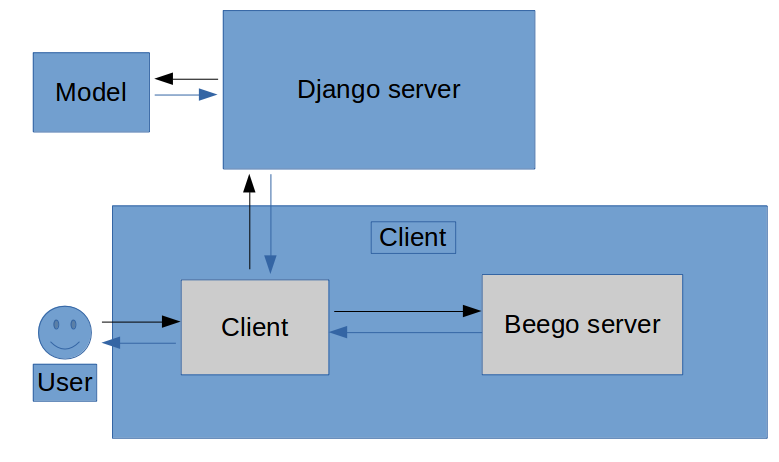
\includegraphics[totalheight=7cm]{Images/app_struct.png}
    \caption{Các thành phần của ứng dụng}
    \label{skip_conn}
\end{figure}
\subsection{RESTful API}
REST(Representational State Transfer) ra đời vào năm 2000 bởi Roy Thomas Fielding có thể gọi đây là các ràng buộc và quy ước mà khi hệ thống nào làm theo thì được gọi là REST.\\
RESTful API là một tiêu chuẩn dùng trong việc thết kế các thiết kế API cho các ứng dụng web để quản lý các resource. RESTful là một trong những kiểu thiết kế API được sử dụng phổ biến nhất ngày nay.\\
Cấu trúc của một RESTful API gồm những phần như sau:
\begin{itemize}
    \item METHOD(Bắt buộc): Gồm các phương thức cơ bản như GET, POST, PUT, DELETE.
    \item URL(Bắt buộc): đường dẫn của API(đường dẫn này sẽ được phân chia trong Routers bên phía server).
    \item DATA(tùy chọn): Đối tượng JSON mô tả dữ liệu kèm theo gửi lên server.
    \item HEADER(Tùy chọn): Một đối tượng JSON thường dùng trong việc bảo mật và xác thực người dùng...
    \item PARAM: Các tham số đi kèm sau dấu "?" của URL.
\end{itemize}
Các bước gọi và phản hồi API cơ bản như sau:\\
Phía client tạo một API chứa những thông tin cần thiết như trên, phía server sẽ kiểm tra header có phù hợp hay không, sau đó nhận dữ liệu, kiểm tra tính hợp lệ của dữ liệu, xử lý và trả lại dữ liệu cần thiết cho client nếu có.
\begin{figure}[h]
\centering
    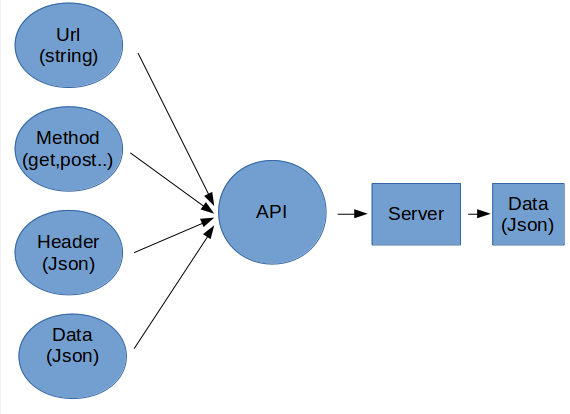
\includegraphics[totalheight=7cm]{Images/app_json.png}
    \caption{Mô tả đơn giản luồng xử lý của một API}
    \label{skip_conn}
\end{figure}
\subsection{Server}
Phần server chính của ứng dụng(Django server) được xây dựng bằng ngôn ngữ Python với framework là Django, làm việc trực tiếp với mô hình đã huấn luyện được và server này sẽ cung cấp một API để client gọi vào. Về framework Django thì chỉ sử dụng để cung cấp và phục vụ một API nên trong báo cáo sẽ không trình bày về các đặc điểm của framework này. Luồng xử lý của server được mô tả như hình bên dưới.
\begin{figure}[h]
\centering
    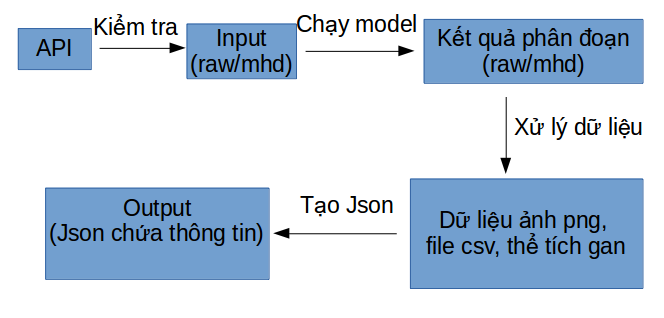
\includegraphics[totalheight=7cm]{Images/app_django_struct.png}
    \caption{Luồng xử lý trong Django server}
    \label{skip_conn}
\end{figure}
\paragraph{Quá trình xử lý dữ liệu đầu vào và chạy model\\}

Dữ liệu đầu vào để server xử lý phải là dữ liệu dưới định dạng raw/mhd(định dạng như tập Sliver07). Dữ liệu có thể chỉ cần tập ảnh scan nếu muốn phân đoạn hoặc bao gồm cả nhãn nếu muốn so sánh và đánh giá kết quả phân đoạn.
Sau khi nhận dữ liệu đầu vào sẽ tiến hành chạy model để cho ra kết quả phân đoạn(Kết quả 1). Đầu ra của quá trình này cũng là file dưới định dạng raw/mhd. Một vài thông tin về quá trình chạy model như sau(cấu hình máy local kèm theo):
\begin{figure}[h]
\centering
    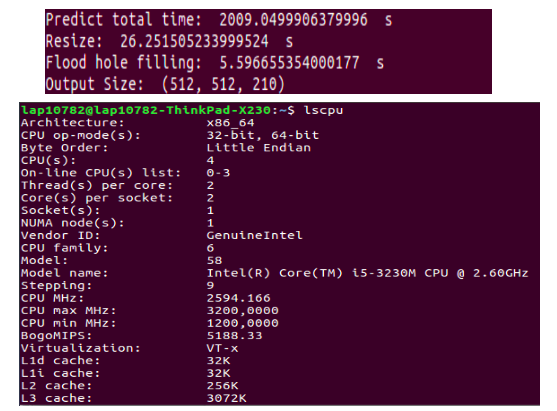
\includegraphics[totalheight=7cm]{Images/app_localinfor.png}
    \caption{Thời gian chạy model của máy tương ứng}
    \label{skip_conn}
\end{figure}
\paragraph{Quá trình hậu xử lý\\}
Tất các các hình ảnh đầu ra đều có định dạng là png.
\begin{itemize}
    \item Với tập đầu vào chỉ có scan, kết quả của quá trình này sẽ bao gồm: Tập ảnh scan, tập ảnh kết quả phân đoạn, tập ảnh phân đoạn dán lên scan, file csv gồm thông tin tập đỉnh và mặt của mô hình gan 3D, thể tích gan theo kết quả phân đoạn.
    \item Với tập có cả scan và nhãn thì kết quả bao gồm: Tập ảnh scan, tập ảnh nhãn, tập ảnh kết quả phân đoạn so sánh với nhãn,  tập ảnh kết quả phân đoạn so sánh với nhãn dán lên scan, file csv gồm thông tin tập đỉnh và mặt mô hình gan 3D và thể tích gan của kết quả phân đoạn và của nhãn.
\end{itemize}
Sau khi tạo các thông tin đó thì tạo file zip kèm theo cho mỗi tập.
\begin{figure}[h]
\centering
    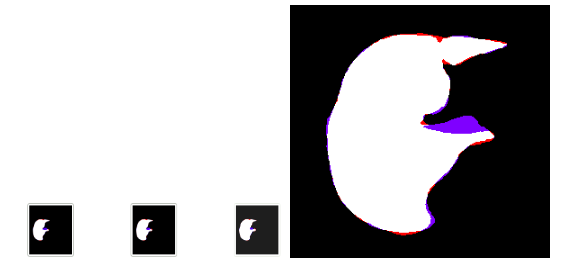
\includegraphics[totalheight=7cm]{Images/app_scancompare.png}
    \caption{Ảnh phân đoạn khi có nhãn}
    \label{skip_conn}
\end{figure}
\begin{figure}[h]
\centering
    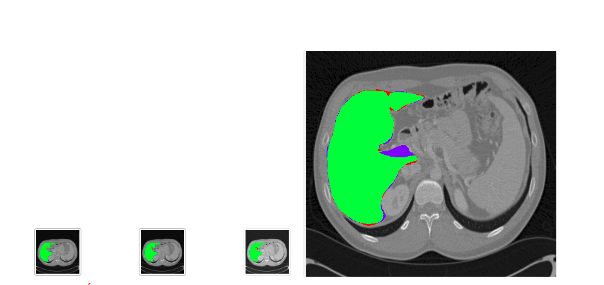
\includegraphics[totalheight=7cm]{Images/app_scanoverlap.png}
    \caption{Ảnh phân đoạn khi có nhãn dán lên scan}
    \label{skip_conn}
\end{figure}
\paragraph{Tạo đối tượng JSON\\}
Với cơ chế gọi API, dữ liệu nhận và gửi sẽ ở định dạng json nên dữ liệu trả về cho client sẽ là một đối tượng json với các trường dữ liệu được mô tả như sau (các đường dẫn tương ứng là các file đã được lưu trong server):
\begin{itemize}
 \item ListPredict: mảng các đường dẫn của ảnh kết quả phân đoạn.
 \item ListLabel: mảng các đường dẫn của ảnh nhãn(nếu có).
 \item ListOverlap: mảng các đường dẫn ảnh kết quả dán lên scan.
 \item CsvFileLabel: đường dẫn tới file csv của nhãn(nếu có).
 \item CsvFilePredict: đường dẫn tới file csv kết quả phân đoạn.
 \item LinkZip: đối tượng JSON chứa các đường dẫn tới file zip của các tập.
 \item VolumePredict: thông tin thể tích theo kết quả phân đoạn.
 \item VolumeLabel: thông tin thể tích nhãn(nếu có).
 \item 
\end{itemize}
Sau khi tạo xong đối tượng JSON sẽ được gửi về client xử lý.
\subsection{Client}
Với cấu trúc server như trên chúng ta có thể xây dựng phần client một cách linh động sao cho trực quan nhất trên bất cứ nền tảng nào qua việc gọi API. Ở phần này thì nhóm xây dựng phần client trên nền tảng website sử dụng framework Beego, với ngôn ngữ phía server là Golang, phía client sử dụng framework là Angularjs để giao tiếp với Golang server.
\begin{figure}[h]
\centering
    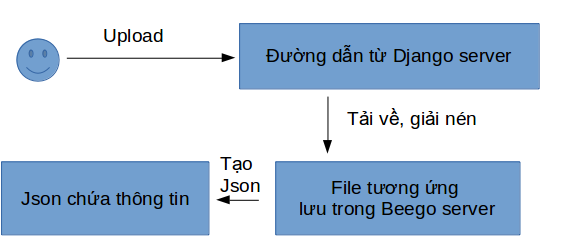
\includegraphics[totalheight=7cm]{Images/app_beego_struct.png}
    \caption{Cấu trúc phần client chính}
    \label{skip_conn}
\end{figure}
\paragraph{Giới thiệu về Golang\\}
Golang hay còn được gọi là Go được thiết kế và phát triển bởi Robert Griesemer, Rob Pike và Ken Thompson tại google vào năm 2007, được giới thiệu vào năm 2009 và hiện tại được sử dụng trong hầu hết trong các sản phẩm của Google. Hiện tại thì Go khá được ưa chuộng bởi các đặc điểm sau:
\begin{itemize}
    \item Hỗ trợ khai báo kiểu dữ liệu động.
    \item Tốc độ biên dịch nhanh.
    \item Hỗ trợ các tác vụ đồng thời.
    \item Ngôn ngữ đơn giản, ngắn gọn.
\end{itemize}
Nói tóm lại, Go có tốc độ xử lý nhanh tương đương như C/C++ nhưng cấu trúc đơn giản và hỗ trợ trình dọn rác tự động nên dễ sử dụng, hiệu quả cao. Để biết thêm thông tin về Go thì có thể tham khảo tại đường dẫn.

\paragraph{Giới thiệu về framework Beego\\}
Beego là một framework open source cho cộng đồng sử dụng miễn phí và phát triển nó theo đường dẫn https://github.com/astaxie/beego.\\
Ta sử dụng beego để tạo một ứng dụng web chạy trực tiếp trên máy chủ local. Khi tạo một dự án bằng Beego ta sẽ được một thư mục có cấu trúc rõ ràng.\\
(Ảnh cây thư mục trong beego).\\
Ứng dụng web được tạo bởi Beego theo mô hình MVC(Model-View-Controller) và giao tiếp qua cơ chế gọi API, các thành phần chính của ứng dụng được giải thích ngắn gọn như sau:\\
\begin{itemize}
    \item Conf: chứa file config định nghĩa một số thông tin chính như cổng, tên, thông tin Database…
    \item Controllers: Nhận và xử lý dữ liệu từ bên ngoài, rồi gọi tới Model và gửi dữ liệu ra nếu có.
    \item Main.go: File để chạy ứng dụng
    \item Models: Nhận dữ liệu đã hợp lệ từ Controllers để xử lý, thường là các tác vụ liên quan tới Database và trả về dữ liệu cần thiết cho Controller.
    \item Routers: Quản lý, phân chia các API cho các Controller tương ứng.
    \item Static: chứa các dữ liệu cần thiết cho phía client.
    \item Tests: Dùng để kiểm tra lại ứng dụng, nơi làm việc của tester.
    \item Views: Mặc định chứa file hiển thị trang chủ.
\end{itemize}
Để tìm hiểu kĩ hơn về framework Beego có thể tham khảo tại: https://beego.me/docs
\paragraph{ Giới thiệu về AngularJS\\}
Angularjs có thể gọi là một framework được viết bằng Javascript. AngularJS đưa ra hướng dẫn cụ thể trên mã lệnh HTML với các tiền tố "ng-" hay còn được gọi là directives.\\
Để sử dụng thì chỉ cần nhúng đường dẫn tới file angular.min.js như sử dụng các thư viện khác.
Một số directive quan trọng có thể kể đến như sau:
\begin{itemize}
    \item ng-app: Đánh dấu thẻ HTML mà AngularJS được bắt đầu sử dụng.
    \item ng-model: giá trị HTML trong thẻ này tương đương với biến \$scope trong phần script.
    \item ng-change, ng-click: bắt sự kiện thay đổi, click để gọi hàm \$scope tương ứng.
\end{itemize}
Một điều quan trọng nữa là AngularJS hỗ trợ gọi API để gửi và nhận dữ liệu một các dễ dàng qua biến \$http.\\
Để biết thêm về AngularJS có thể tham khảo tại 

\paragraph{Một số thư viện hỗ trợ khác được sử dụng\\}
\begin{itemize}
    \item Bootstrap: Thư viện quen thuộc để xây dựng giao diện responsive dễ dàng. Trong ứng dụng này sử dụng bootstrap phiên bản 3.3.7.
    \item Plotly: Thư viện giúp hiển thị hình ảnh 3D từ file csv chứa tập đỉnh và mặt.
    \item Jquery, Font Awesome, Rangesslider hỗ trợ việc hiển thị được tốt và hiệu quả hơn.
\end{itemize}

\paragraph{Luồng xử lý bên phía client của ứng dụng\\}
Như đã nên trên, bên phía client của ứng dụng cũng sẽ có client-server nữa để thực hiện việc hiển thị và lưu lại kết quả gần nhất. Ta tạm gọi server chính là Django-server và server phụ là Beego-server. Luồng xử lý của phần client này được mô tả như sau:\\
Sau khi upload dữ liệu cho Django-server qua một API, client sẽ nhận về các thông tin của server này đồng thời gửi lại cho Beego-server, sau đó Beego-server sẽ lấy những đường dẫn chứa file zip giải nén và lưu vào thư mục của nó đồng thời tạo file lưu thông tin thể tích lá gan sau đó gửi cho client đường dẫn là các file được lưu trong Beego-server. Client sẽ thực hiện việc hiển thị kết quả từ những đường dẫn này. Khi khởi động ứng dụng lên, client sẽ gọi API cho Beego-server để lấy lại những đường dẫn này. Sau khi có được đường dẫn thì hiển thị kết quả, dùng thư viện đọc file để hiển thị mô hình 3D. Phần này sẽ được trình bày trực quan ở mục 9.2.
\section{Các chức năng và kết quả hiển thị của ứng dụng.}
Về phần hiển thị, trang web được xây dựng khá đơn giản nhưng đảm bảo được những thông tin cần thiết của kết quả phân đoạn một lá gan.
\subsection{Trang giới thiệu.}
Trang này chỉ đơn giản là giới thiệu về chức năng của website.
\begin{figure}[h]
\centering
    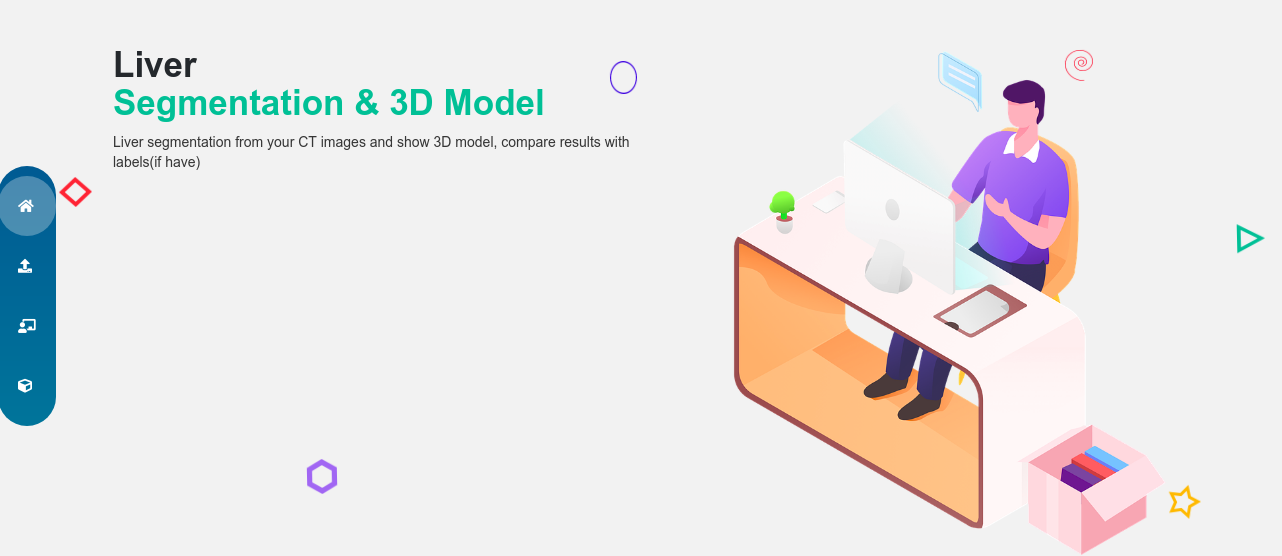
\includegraphics[totalheight=7cm]{Images/app_intro.png}
    \caption{Giao diện trang giới thiệu ứng dụng}
    \label{skip_conn}
\end{figure}
\subsection{Trang upload dữ liệu}
Trang này cho phép người dùng upload dữ liệu lên. Dữ liệu là tập scan có định dạng raw/mhd được nén trực tiếp ở dạng zip. Sau khi upload thì đợi kết quả trả về(chạy trên máy local mất khoảng 30 phút). Nếu dữ liệu có thêm label thì kết quả trả về có dạng để so sánh. Kết quả sẽ được hiển thị ở trang tiếp theo.
\begin{figure}[h]
\centering
    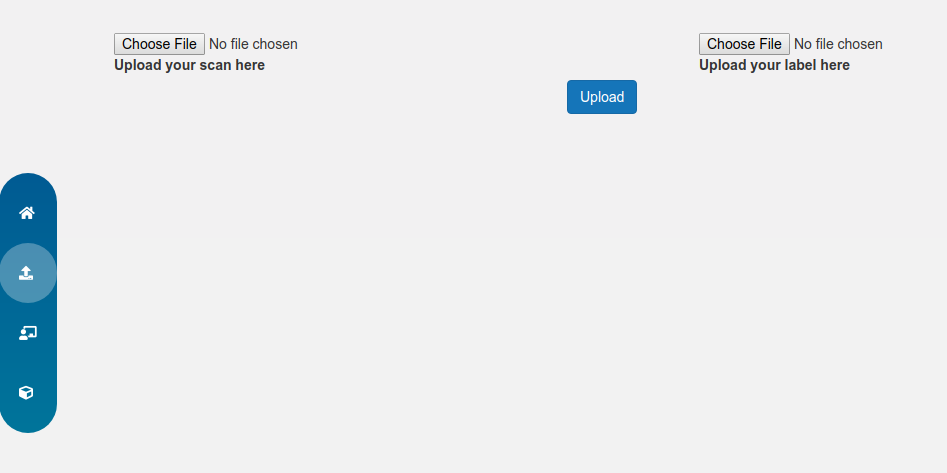
\includegraphics[totalheight=7cm]{Images/app_upload.png}
    \caption{Giao diện trang upload dữ liệu}
    \label{skip_conn}
\end{figure}
\subsection{Trang hiển thị kết quả phân đoạn}
Như đã nêu trên, nếu dữ liệu upload chỉ có scan, thì trang này hiển thị 3 mục như sau:
\begin{itemize}
    \item Ảnh scan(ảnh gốc lúc upload).
    \item Ảnh phân đoạn gan.
    \item Ảnh phân đoạn dán lên scan tương ứng.
\end{itemize}

\begin{figure}[h]
\centering
    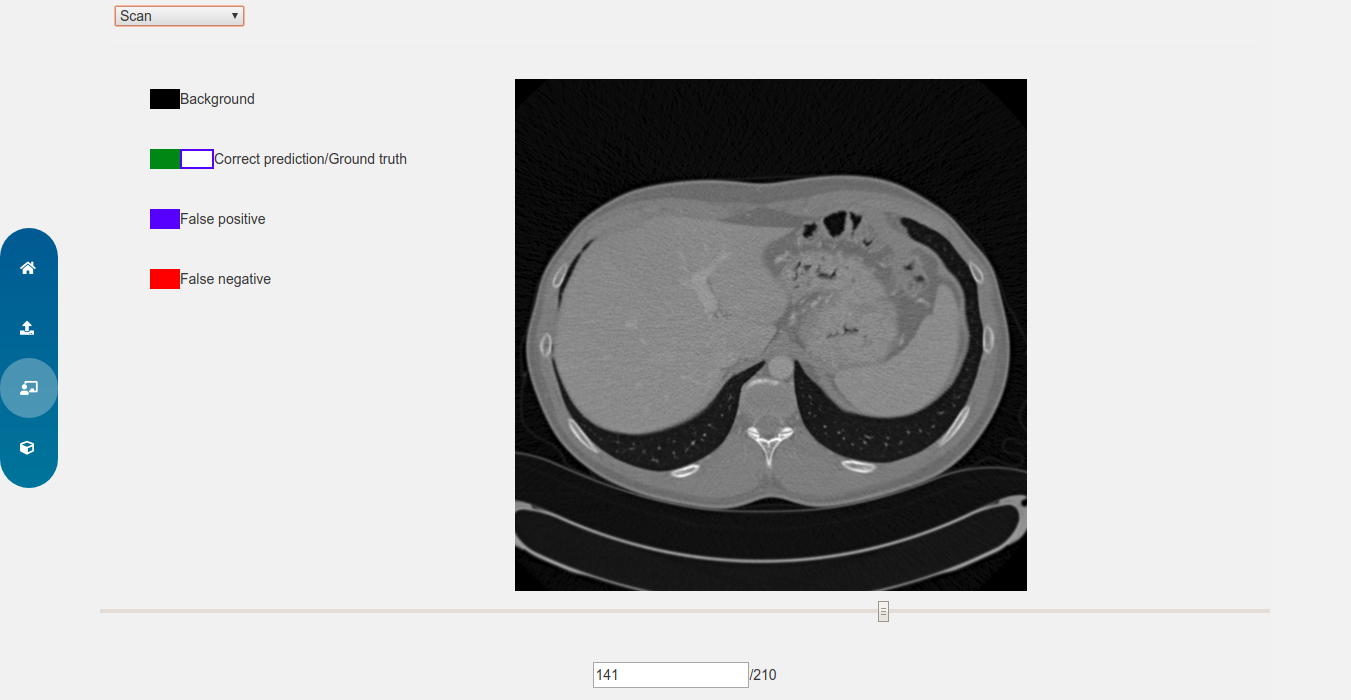
\includegraphics[totalheight=7cm]{Images/app_scan.png}
    \caption{Hiển thị ảnh scan}
    \label{skip_conn}
\end{figure}
\begin{figure}[h]
\centering
    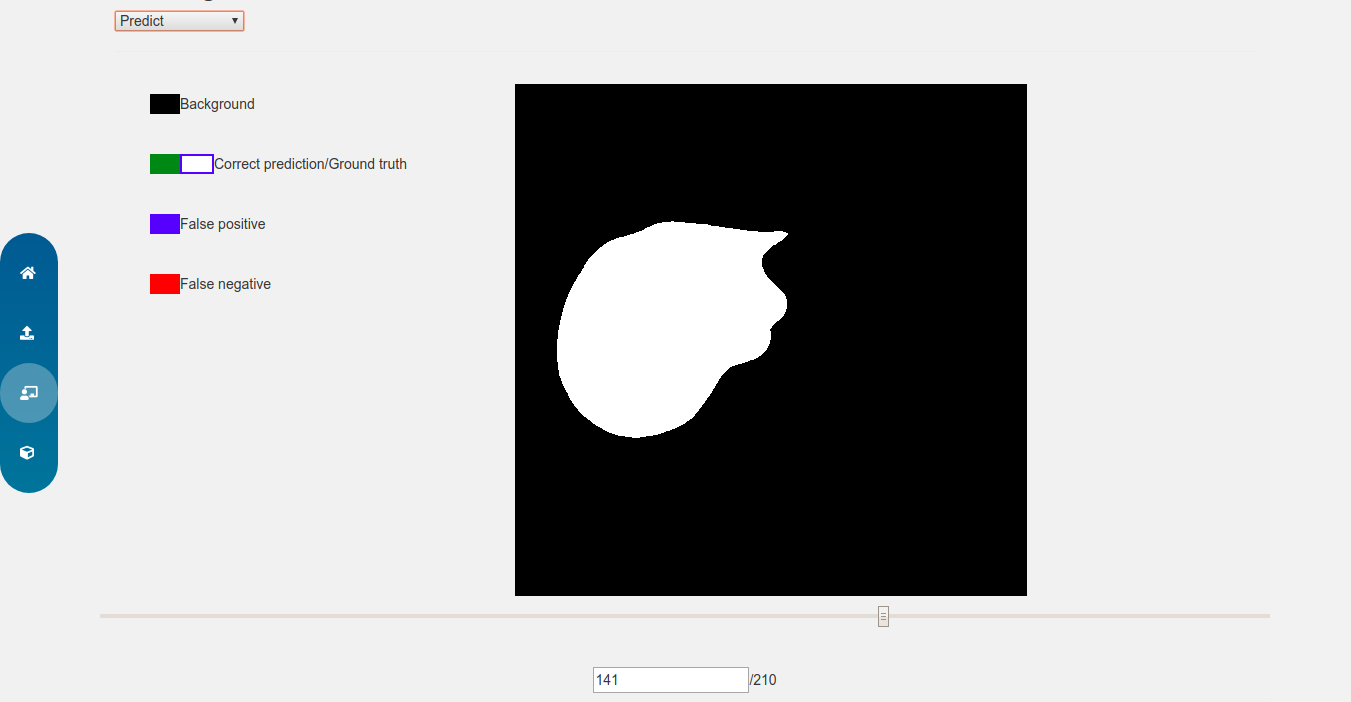
\includegraphics[totalheight=7cm]{Images/app_label.png}
    \caption{Hiển thị ảnh phân đoạn khi không có nhãn}
    \label{skip_conn}
\end{figure}
\begin{figure}[h]
\centering
    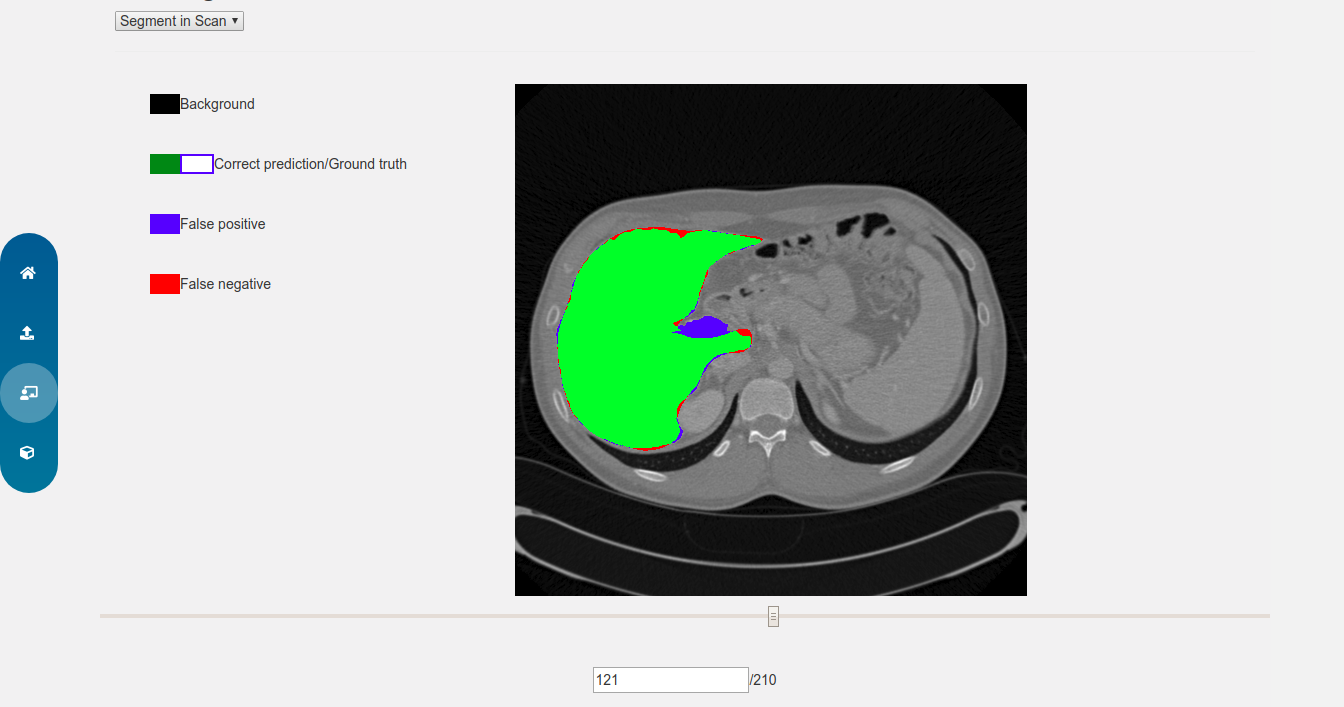
\includegraphics[totalheight=7cm]{Images/app_overlap_1.png}
    \caption{Hiển thị ảnh phân đoạn dán lên scan}
    \label{skip_conn}
\end{figure}
Nếu tập dữ liệu có thêm nhãn thì kết quả hiển thị có ảnh scan giống với mục trên, các ảnh còn lại sẽ là kết quả để so sánh với nhãn.
\begin{figure}[h]
\centering
    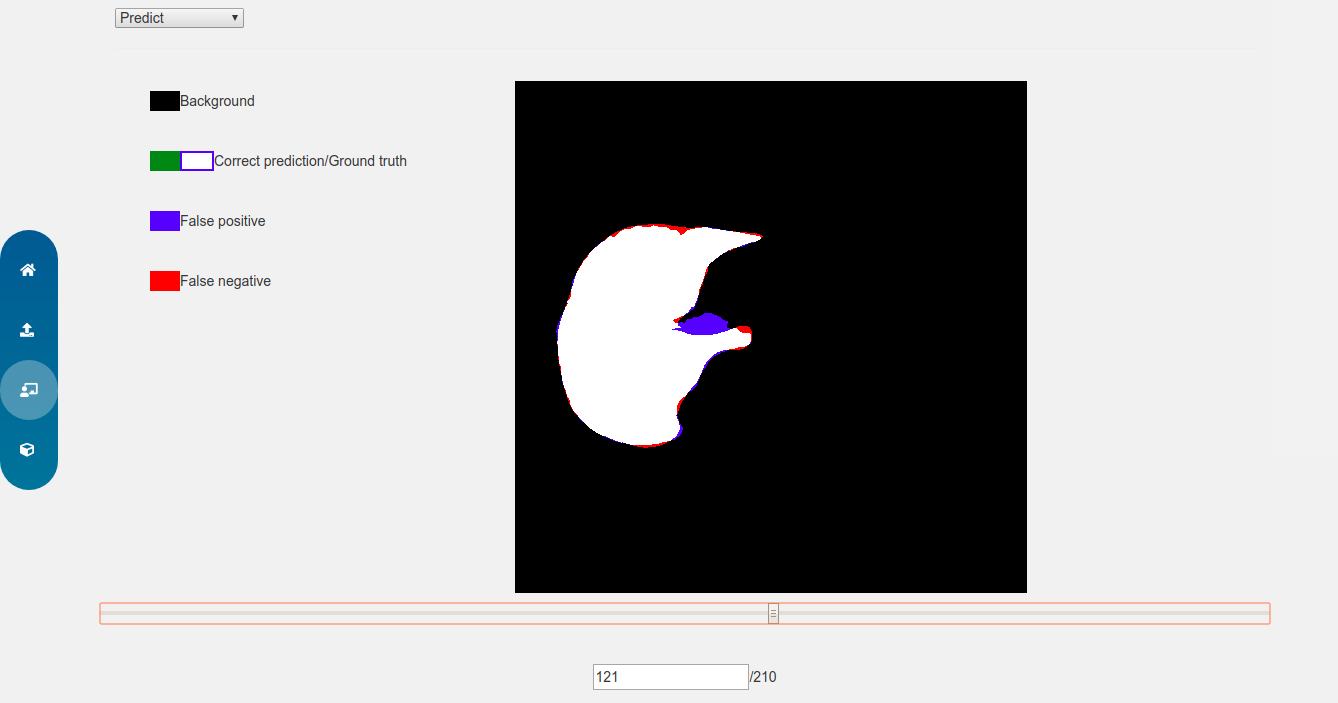
\includegraphics[totalheight=7cm]{Images/app_showscanompare.png}
    \caption{Hiển thị ảnh phân đoạn so sánh với nhãn}
    \label{skip_conn}
\end{figure}
\begin{figure}[h]
\centering
    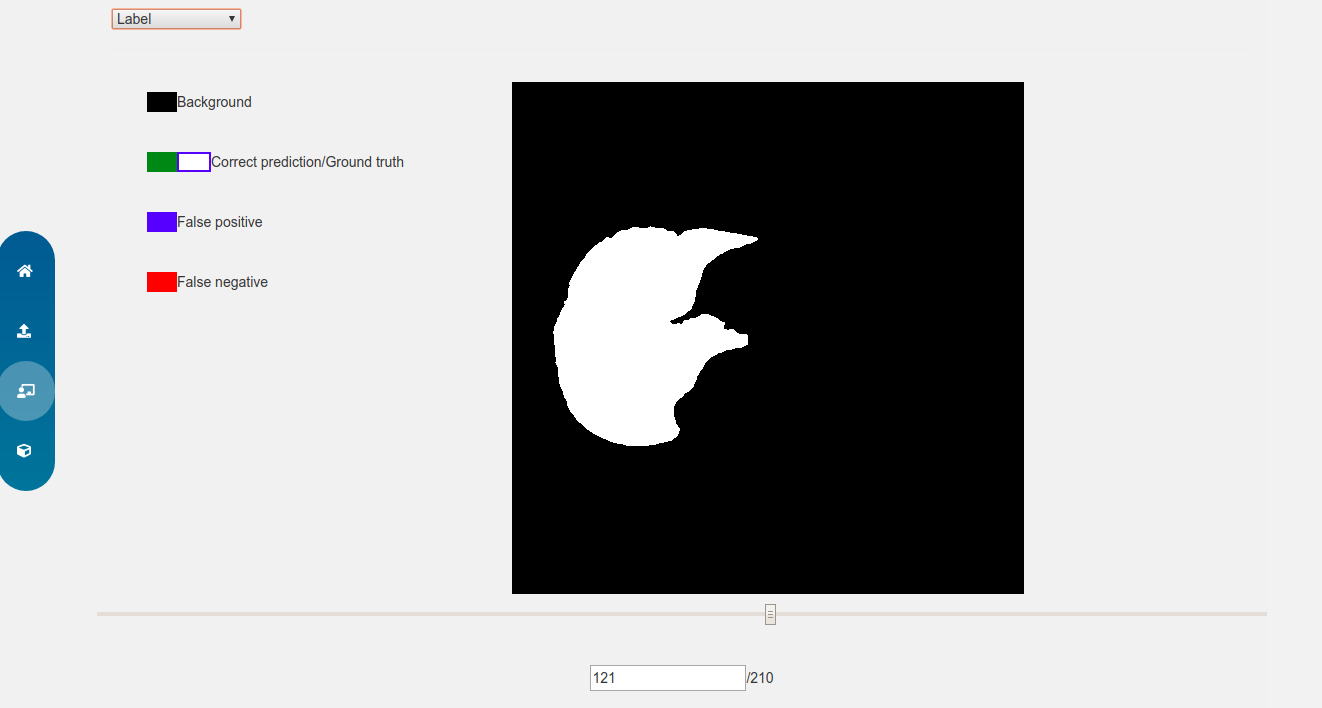
\includegraphics[totalheight=7cm]{Images/app_labelreal.png}
    \caption{Hiển thị ảnh nhãn}
    \label{skip_conn}
\end{figure}
\begin{figure}[h]
\centering
    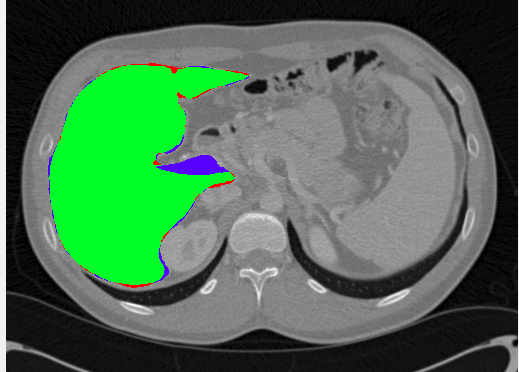
\includegraphics[totalheight=7cm]{Images/app_overlap_2.png}
    \caption{Hiển thị ảnh phân đoạn so sánh với nhãn dán lên scan}
    \label{skip_conn}
\end{figure}

\subsection{Trang hiển thị mô hình 3D}
Trang này hiển thị mô hình 3D bằng cách dùng thư viện plotly.js đọc file csv được tạo ra trong Django server đồng thời hiển thị thể tích của gan. Người dùng có thể dùng chuột để xoay, thu nhỏ, phóng to để xem chi tiết mô hình.
\begin{figure}[h]
\centering
    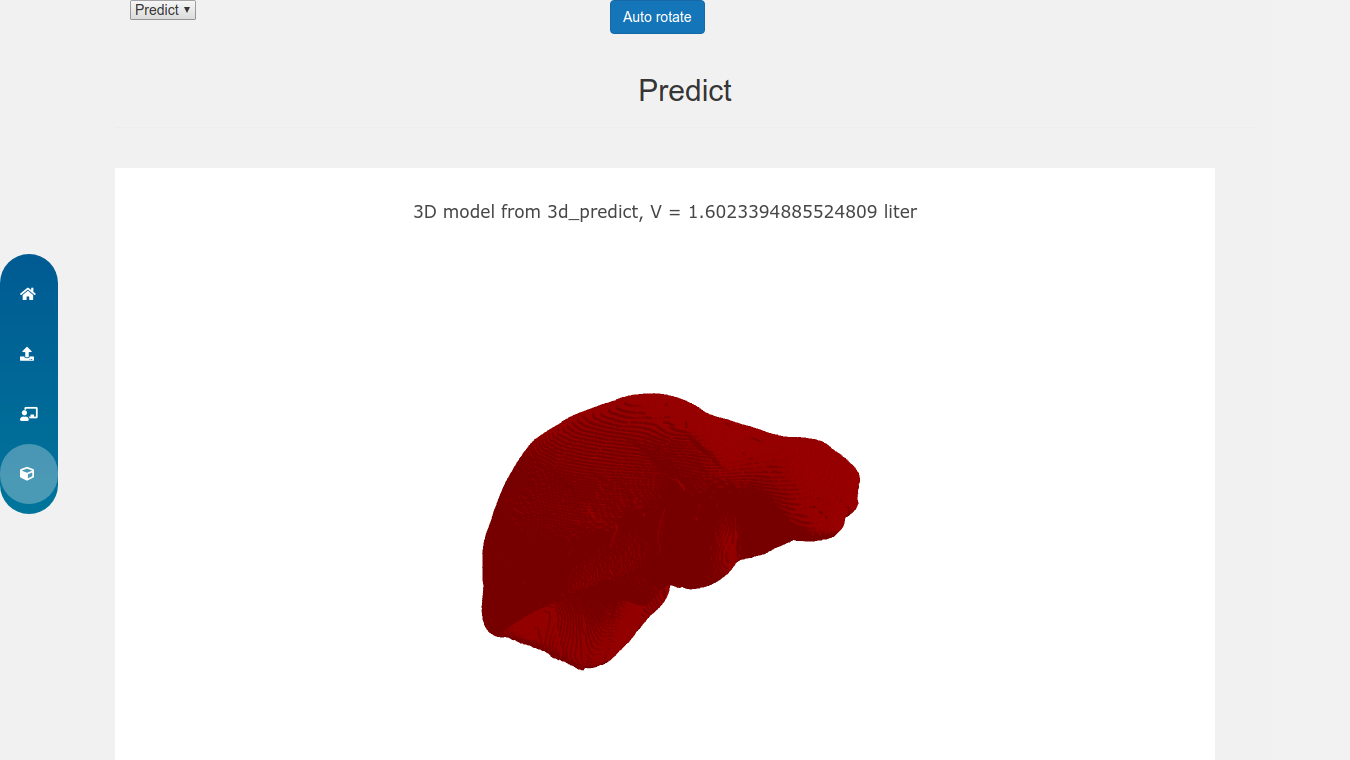
\includegraphics[totalheight=7cm]{Images/app_3dpredict.png}
    \caption{Hiển thị mô hình 3D dự đoán kèm thể tích}
    \label{skip_conn}
\end{figure}
\begin{figure}[h]
\centering
    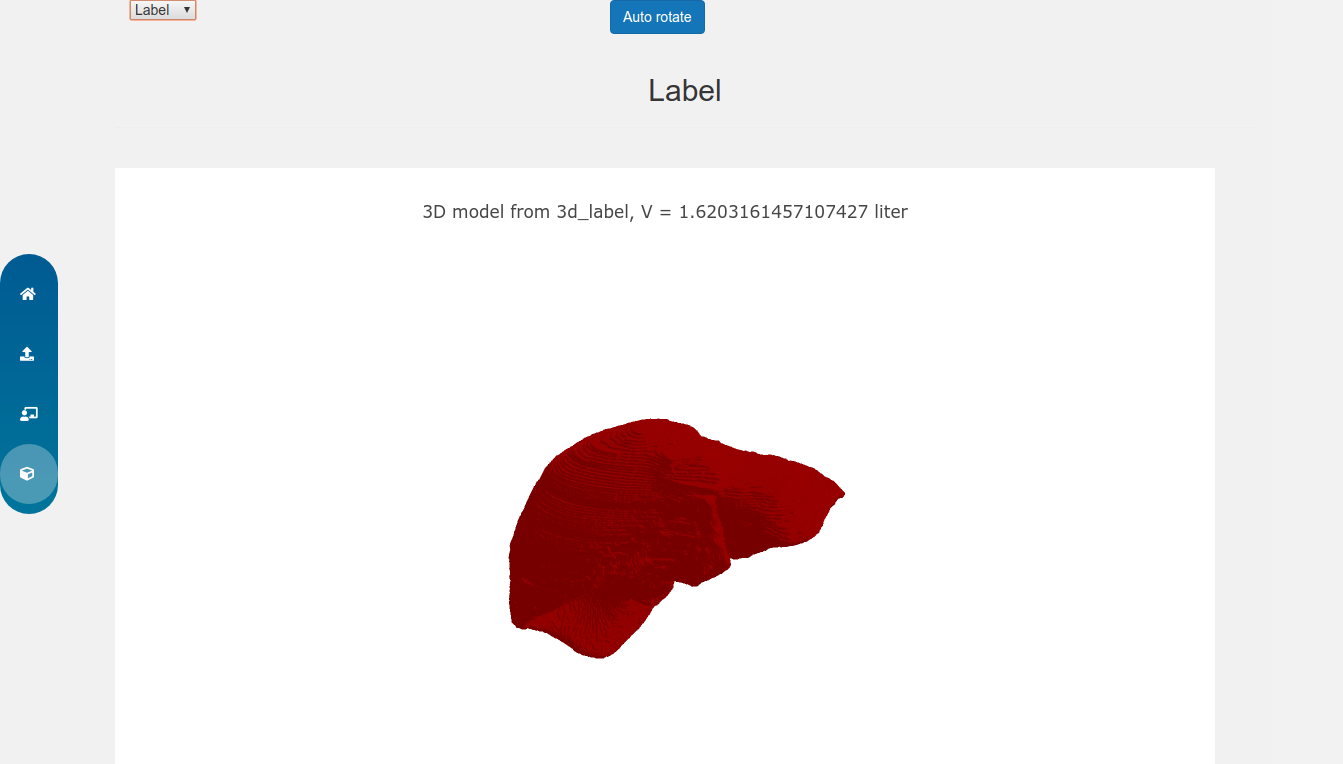
\includegraphics[totalheight=7cm]{Images/app_3dlabel.png}
    \caption{Hiển thị mô hình 3D của nhãn kèm thể tích}
    \label{skip_conn}
\end{figure}

Ta có thể click vào nút "Auto rotate" để lá gan xoay tự động. Một mô hình sẽ có khoảng hai trăm nghìn điểm và bốn trăm nghìn mặt nên chức năng tự động xoay khá chậm.
\section{Ưu nhược điểm của ứng dụng}
Ưu điểm:\\
\begin{itemize}
    \item Các thành phần được xây dựng riêng biệt với nhau nên dễ dàng sửa đổi và phát triển.
    \item Mô hình 3D dễ dàng điều chỉnh để xem chi tiết lá gan.
\end{itemize}
Nhược điểm:\\
\begin{itemize}
    \item Chưa có bảo mật.
    \item Giao diện còn khá đơn giản.
\end{itemize}
